A network is useful not only because it connects, but because it connects in more than one way. 
A single road between two towns is a liability and a second independent road is insurance. 
The mathematical content of that intuition is the number of routes between two points that share no segment and the question this thesis circles is how many connections a network can hold before some pair of points is forced to have too many such routes. 
This chapter gives the foundation for the question and its variants and goes over the results that can be proven using logical arguments. 

\section{Graphs and routes}

To state the question precisely we need only a few ideas. 
A \emph{graph} $G$ is a finite set of points, called \emph{vertices}, together with a (multi)set of \emph{edges}, each joining two (or more) distinct vertices. 
We write $V(G)$ for the set of vertices and $E(G)$ for the (multi)set of edges. 
Therefore $|E(G)|$ is the number of edges, which is the very quantity this thesis tries to make as large as possible under certain constraints.
If $E(G)$ is a set and its edges join exactly two vertices, $G$ is a \emph{simple graph}.
One pictures such a simple graph by representing the vertices as dots and the edges as lines between them.

\begin{figure}[ht]
\centering
\begin{tikzpicture}[scale=1.0,
    mv/.style={gvertex},
    me/.style={gline}]
  \foreach \i in {0,...,4} {
    \pgfmathsetmacro{\ang}{90 + 72*\i}
    \coordinate (v\i) at (\ang:1.4);
  }
  \draw[me] (v0)--(v1) (v0)--(v2) (v0)--(v3)
            (v1)--(v2) (v1)--(v4)
            (v2)--(v3) (v2)--(v4)
            (v3)--(v4);
  \foreach \i in {0,...,4} {
    \pgfmathsetmacro{\ang}{90 + 72*\i}
    \node[mv] at (\ang:1.4) {$\i$};
  }
\end{tikzpicture}
\caption{The simple graph $K_5-\{04,13\}$ has five vertices and eight edges, where $K_n$ is the complete graph on $n$ vertices.}
\label{fig:k5-example}
\end{figure}

We write $n\coloneq|V(G)|$ for the number of vertices and define the \emph{degree} of a vertex as the number of edges meeting it. 
Unless specified otherwise, graphs are simple.
A \emph{path} from a vertex $u$ to a vertex $v$ is a sequence of distinct vertices that starts at $u$, ends at $v$, and joins each consecutive pair by an edge. 
Two paths between the same endpoints are \emph{edge-disjoint} if no edge belongs to both.
The largest number of pairwise edge-disjoint paths between $u$ and $v$ is their \emph{local edge-connectivity} $\lec_G(u, v)$. 
The pair with the most such paths sets the ceiling for the whole graph:
\[
    \lec_G^{\max} = \max_{u \ne v} \lec_G(u, v).
\]
A theorem of Menger \cite{Menger27}, recalled in \Cref{app:proofs}, gives this quantity a second face: $\lec_G(u, v)$ also equals the least number of edges one must remove to cut every route from $u$ to $v$ (\Cref{fig:menger}). 
Edge disjoint paths between a pair is exactly the same thing as the minimum cut of unit flow between them.

\begin{figure}[ht]
\centering
\begin{tikzpicture}[scale=1.2,
    mv/.style={gvertex},
    me/.style={gline},
    rA/.style={grA},
    rB/.style={grB},
    rC/.style={grC},
    cut/.style={gcutedge}]
  \foreach \i in {0,...,4} {
    \pgfmathsetmacro{\ang}{90 + 72*\i}
    \coordinate (v\i) at (\ang:1.5);
  }
  % all eight edges, faint background
  \draw[me] (v0)--(v1) (v0)--(v2) (v0)--(v3)
            (v1)--(v2) (v1)--(v4)
            (v2)--(v3) (v2)--(v4)
            (v3)--(v4);
  % three edge-disjoint routes between the non-adjacent pair 1 and 3
  \draw[rA] (v1)--(v0)--(v3);
  \draw[rB] (v1)--(v2)--(v3);
  \draw[rC] (v1)--(v4)--(v3);
  % minimum cut: the three edges meeting vertex 1, a dashed ring around it
  \draw[cut] (v1) circle (0.6);
  \node[vertexred, font=\scriptsize] at (-1.35,1.55) {cut: $3$ edges};
  \foreach \i in {0,...,4} {
    \pgfmathsetmacro{\ang}{90 + 72*\i}
    \node[mv] at (\ang:1.5) {$\i$};
  }
\end{tikzpicture}
\caption{Menger's theorem on \Cref{fig:k5-example}: three edge-disjoint $1$--$3$ routes (coloured) meet the minimal three-edge cut around vertex $1$, so $\lec(1,3)=3$.}
\label{fig:menger}
\end{figure}

\section{Erd\H{o}s Problem 915}

The constraint at the heart of this thesis is a ceiling on connectivity. 
Requiring $\lec_G^{\max} \le m - 1$ says that no pair of vertices is joined by as many as $m$ edge-disjoint paths, or equivalently that every pair can be severed by removing fewer than $m$ edges. 
The question is how many edges a graph can hold while staying under that ceiling.

\begin{ques}[Erd\H{o}s Problem 915 \cite{ErdosProblems}]
How many edges can a graph on $n$ vertices have if no two of its vertices are joined by $m$ edge-disjoint paths?
\end{ques}

Writing the answer as an extremal function,
\[
    \ell_m(n) = \max\{\, |E(G)| : |V(G)| = n,\ \lec_G^{\max} \le m - 1 \,\},
\]
the problem asks for $\ell_m(n)$, the most edges possible under the ceiling. 
Mader proved that no graph under the ceiling has more than $\floor{m(n-1)/2}$ edges (the upper bound) in the simple-graph case and provided the shared-clique construction, which achieves the bound but is only defined when $m-1$ divides $n-1$.
The brackets $\floor{\,\cdot\,}$ round their content down to the nearest whole number and their ceiling counterpart $\ceil{\,\cdot\,}$ rounds up. Both recur throughout, because an edge count is always an integer while the formulas that bound it need not be.

\begin{theorem}[Mader \cite{Mader73}]\label{thm:mader}
For all $n \ge m \ge 2$,
\[
    \ell_m(n) \le \floorfrac{m(n-1)}{2}.
\]
\end{theorem}

Notice how $n \ge m$ is not needed here, but will be to attain equality since simple graphs cannot exceed the edge count of complete graphs. 
The proof given in \Cref{app:proofs} was discovered independently of Mader and uses the Gomory-Hu tree (\Cref{thm:gomory-hu}). 
The shared clique graph is then generalised to an extremal construction that exists for all values of $n\ge m$ (\Cref{thm:extremal-char}). 
The very same Gomory-Hu tree returns for the multigraph and hypergraph variants (\Cref{thm:multigraph-edge}, \Cref{prop:hyper-edge}). 
Hence it is worth mentioning its properties here.
Every graph has a weighted, spanning tree such that $\lec_G(u, v)$ equals the lightest edge on the tree path from $u$ to $v$.
All $\binom{n}{2}$ local connectivities are therefore encoded by just $n - 1$ weights. 
The largest of them, $\lec_G^{\max}$, is simply the heaviest edge of the tree. 
The proof (\Cref{app:proofs}) uses a double counting argument on that tree. 

\section{Variants of the problem}

So far the problem has been stated for simple graphs, but the same question remains unanswered in a more general setting.
Each assumption made so far will be toggled to create a lattice of variants and the thesis will explore each node of that lattice.

The first is \emph{arity}: an edge joins exactly two vertices and a \emph{hyperedge} joins $r \ge 2$.
Hence such \emph{hypergraphs} use \emph{Berge paths}, which aligns with the path definition above.
The second is \emph{multiplicity}: a \emph{simple} graph carries at most one copy of each edge, while a \emph{multi} graph allows parallel copies, recorded by a multiplicity $\mu(u, v)$.
The third is \emph{direction}: a directed edge, called arc, is an ordered pair of vertices and a directed hyperedge has one tail and $r-1$ heads.
These three toggles create a lattice of eight models, shown in \Cref{fig:eight-models}.

\begin{figure}[ht]
\centering
\resizebox{\textwidth}{!}{%
\begin{tikzpicture}[>=Stealth,
    mv/.style={gvertex, minimum size=5.5mm},
    me/.style={gline},
    ml/.style={metro, line width=2.8pt},
    stn/.style={metrostop, minimum size=5mm},
    darc/.style={gdir},
    hstar/.style={metro, line width=2.7pt, -{Stealth[length=2.8mm]}, shorten >=3.2mm, shorten <=2.4mm}]
  % (a) simple graph: K_3 triangle, single edges only
  \begin{scope}[shift={(0,0)}]
    \node[mv] (s1) at (90:0.78) {};
    \node[mv] (s2) at (210:0.78) {};
    \node[mv] (s3) at (330:0.78) {};
    \draw[me] (s1)--(s2)  (s2)--(s3)  (s3)--(s1);
    \node[font=\itshape] at (0,-1.75) {simple graph};
    \node[font=\scriptsize, text=black!65] at (0,-2.25) {one edge per pair};
  \end{scope}
  % (b) multigraph: K_3 with a triple edge and a double edge, the third single
  \begin{scope}[shift={(4.30,0)}]
    \node[mv] (g1) at (90:0.78) {};
    \node[mv] (g2) at (210:0.78) {};
    \node[mv] (g3) at (330:0.78) {};
    % triple edge on the left side
    \draw[me] (g1) to[bend left=22] (g2);
    \draw[me] (g1) -- (g2);
    \draw[me] (g1) to[bend right=22] (g2);
    % double edge on the bottom side
    \draw[me] (g2) to[bend left=15] (g3);
    \draw[me] (g2) to[bend right=15] (g3);
    % single edge on the right side
    \draw[me] (g3) -- (g1);
    \node[font=\itshape] at (0,-1.75) {multigraph};
    \node[font=\scriptsize, text=black!65] at (0,-2.25) {parallel edges $\mu(u,v)\!\ge\!1$};
  \end{scope}
  % (c) simple hypergraph: three distinct size-3 hyperedges, metro-style, on the
  %     four corner stations (no central station). Two share the bottom stretch
  %     and run parallel side by side there; the third runs diagonally corner to
  %     corner. No hyperedge is repeated.
  \begin{scope}[shift={(8.60,0)}]
    \coordinate (A) at (-0.85,-0.85); \coordinate (B) at (0.85,-0.85);
    \coordinate (C) at (0.85, 0.85);  \coordinate (D) at (-0.85,0.85);
    \begin{scope}[on background layer]
      % {A,B,C}: bottom (upper offset) + right
      \draw[ml, metroB] (-0.85,-0.77) -- (0.85,-0.77) -- (0.85,0.85);
      % {A,B,D}: left + bottom (lower offset), parallel to the blue line on the bottom
      \draw[ml, metroC] (-0.85,0.85) -- (-0.85,-0.93) -- (0.85,-0.93);
      % {A,C,D}: diagonal A--C + top C--D
      \draw[ml, metroD] (-0.85,-0.85) -- (0.85,0.85) -- (-0.85,0.85);
    \end{scope}
    \foreach \p in {A,B,C,D} {\node[stn] at (\p) {};}
    \node[font=\itshape] at (0,-1.75) {hypergraph};
    \node[font=\scriptsize, text=black!65] at (0,-2.25) {hyperedges span $r\!\ge\!3$};
  \end{scope}
  % (d) multi-hypergraph: one repeated hyperedge {A,B,C} (two parallel red lines
  %     side by side, the hypergraph counterpart of parallel edges) plus one
  %     ordinary, non-repeated hyperedge {B,C,D} drawn diagonally corner to
  %     corner. No central station.
  \begin{scope}[shift={(12.90,0)}]
    \coordinate (A) at (-0.85,-0.85); \coordinate (B) at (0.85,-0.85);
    \coordinate (C) at (0.85, 0.85);  \coordinate (D) at (-0.85,0.85);
    \begin{scope}[on background layer]
      \draw[ml, metroA] (-0.85,-0.93) -- (0.93,-0.93) -- (0.93,0.85);   % {A,B,C}
      \draw[ml, metroA] (-0.85,-0.77) -- (0.77,-0.77) -- (0.77,0.85);   % {A,B,C} repeated
      \draw[ml, metroB] (0.85,-0.85) -- (-0.85,0.85) -- (0.85,0.85);    % {B,C,D} diagonal, single
    \end{scope}
    \foreach \p in {A,B,C,D} {\node[stn] at (\p) {};}
    \node[font=\itshape] at (0,-1.75) {multi-hypergraph};
    \node[font=\scriptsize, text=black!65] at (0,-2.25) {a hyperedge repeated};
  \end{scope}
  % (a) simple digraph: directed triangle with one bidirected pair
  \begin{scope}[shift={(0,-4.5)}]
    \node[mv] (s1d) at (90:0.78) {};
    \node[mv] (s2d) at (210:0.78) {};
    \node[mv] (s3d) at (330:0.78) {};
    % directed 3-cycle, every arc bowing slightly outward, plus one back arc
    \draw[darc] (s1d) to[bend right=14] (s2d);
    \draw[darc] (s2d) to[bend right=14] (s3d);
    \draw[darc] (s3d) to[bend right=14] (s1d);
    \draw[darc] (s2d) to[bend right=14] (s1d);
    \node[font=\itshape] at (0,-1.75) {simple digraph};
    \node[font=\scriptsize, text=black!65] at (0,-2.25) {one arc per ordered pair};
  \end{scope}
  % (b) directed multigraph: a triple arc, a bidirected pair, a single arc
  \begin{scope}[shift={(4.3,-4.5)}]
    \node[mv] (g1d) at (90:0.78) {};
    \node[mv] (g2d) at (210:0.78) {};
    \node[mv] (g3d) at (330:0.78) {};
    % g1 -> g2: a triple of parallel arcs, fanned outward and well spaced
    \draw[darc] (g1d) to[bend left=22] (g2d);
    \draw[darc] (g1d) to[bend right=0] (g2d);
    \draw[darc] (g1d) to[bend right=22] (g2d);
    % g2 <-> g3: opposite arcs (bidirected)
    \draw[darc] (g2d) to[bend right=12] (g3d);
    \draw[darc] (g3d) to[bend right=12] (g2d);
    % g3 -> g1: single, outward
    \draw[darc] (g3d) to[bend right=14] (g1d);
    \node[font=\itshape] at (0,-1.75) {directed multigraph};
    \node[font=\scriptsize, text=black!65] at (0,-2.25) {parallel and opposite arcs};
  \end{scope}
  % (c) directed hypergraph: the SAME three hyperedges as fig:four-models,
  %     {A,B,C} blue, {A,B,D} green, {A,C,D} orange. Each is a metro-styled star
  %     whose tail is the MIDDLE station of the undirected line, so the arcs land
  %     on the very same edges. Blue and green share the bottom edge, one arc each
  %     way (opposite directions -> SAME bend, so they straddle the edge).
  \begin{scope}[shift={(8.6,-4.5)}]
    \coordinate (Ad) at (-0.85,-0.85); \coordinate (Bd) at (0.85,-0.85);
    \coordinate (Cd) at (0.85, 0.85);  \coordinate (Dd) at (-0.85,0.85);
    \begin{scope}[on background layer]
      % blue {A,B,C}, tail B: B->A (bottom) + B->C (right)
      \draw[hstar, metroB] (Bd) to[bend left=16] (Ad);
      \draw[hstar, metroB] (Bd) to (Cd);
      % green {A,B,D}, tail A: A->B (bottom, opposite blue, same bend) + A->D (left)
      \draw[hstar, metroC] (Ad) to[bend left=16] (Bd);
      \draw[hstar, metroC] (Ad) to (Dd);
      % orange {A,C,D}, tail C: C->A (diagonal) + C->D (top)
      \draw[hstar, metroD] (Cd) to (Ad);
      \draw[hstar, metroD] (Cd) to (Dd);
    \end{scope}
    \foreach \p in {Ad,Bd,Cd,Dd} {\node[stn] at (\p) {};}
    \node[font=\itshape] at (0,-1.75) {directed hypergraph};
    \node[font=\scriptsize, text=black!65] at (0,-2.25) {two share an edge};
  \end{scope}
  % (d) directed multi-hypergraph: the SAME two hyperedges as fig:four-models,
  %     {A,B,C} red repeated and {B,C,D} blue, as metro stars on the same edges
  %     (tail = middle station). Each repeated arc is a parallel pair (same
  %     direction -> OPPOSITE bends, so the pair straddles the edge).
  \begin{scope}[shift={(12.9,-4.5)}]
    \coordinate (Am) at (-0.85,-0.85); \coordinate (Bm) at (0.85,-0.85);
    \coordinate (Cm) at (0.85, 0.85);  \coordinate (Dm) at (-0.85,0.85);
    \begin{scope}[on background layer]
      % red {A,B,C}, tail B, repeated: B->A and B->C, each a straddling pair
      \draw[hstar, metroA] (Bm) to[bend left=16] (Am);
      \draw[hstar, metroA] (Bm) to[bend right=16] (Am);
      \draw[hstar, metroA] (Bm) to[bend left=16] (Cm);
      \draw[hstar, metroA] (Bm) to[bend right=16] (Cm);
      % blue {B,C,D}, tail D: D->B (diagonal) + D->C (top)
      \draw[hstar, metroB] (Dm) to (Bm);
      \draw[hstar, metroB] (Dm) to (Cm);
    \end{scope}
    \foreach \p in {Am,Bm,Cm,Dm} {\node[stn] at (\p) {};}
    \node[font=\itshape] at (0,-1.75) {directed multi-hypergraph};
    \node[font=\scriptsize, text=black!65] at (0,-2.25) {a hyperedge repeated};
  \end{scope}
\end{tikzpicture}}
\caption{The eight models side by side, with the four undirected on top and the four directed below. The simple graph is a triangle, the multigraph has parallel edges, the hypergraph has three hyperedges, and the multi-hypergraph has one repeated hyperedge. The directed versions have arcs instead of edges, with the same pattern of repetition and hyperedges.}
\label{fig:eight-models}
\end{figure}

The digraphs do not have a Gomory-Hu tree, but they do have a directed analogue of Menger's theorem.
A digraph has three degree counts at each vertex. The \emph{out-degree} $d^+(v)$ counts the arcs leaving $v$ and the vertices they reach are its \emph{out-neighbours}. 
The \emph{in-degree} $d^-(v)$ counts the arcs entering $v$ and the vertices they come from are its \emph{in-neighbours}. 
The \emph{total degree} $d(v) = d^+(v) + d^-(v)$ adds the two. 
\Cref{fig:directed-lambda} shows a digraph carrying three arc-disjoint routes between one chosen pair of vertices. 
The directed form of Menger's theorem says that route count equals the size of the smallest arc-cut separating the pair, and the figure also marks the out-degree and in-degree that bound both quantities from above, which is exactly how Menger reads in a one-way network.
A directed $r$-edge has one tail and $r-1$ heads. 
In the figures, one colour denotes one hyperedge, drawn either as a star or as a line oriented away from its tail. 
It is a single edge on several vertices, not a path of ordinary edges. 
A directed \emph{Berge route} enters that edge at its tail and leaves at one of its heads.

\begin{figure}[ht]
\centering
\begin{tikzpicture}[>=Stealth, scale=1.2,
    mv/.style={gvertex},
    me/.style={gdirfaint, shorten >=3.5mm},
    rA/.style={grAd, shorten >=3.5mm},
    rB/.style={grBd, shorten >=3.5mm},
    rC/.style={grCd, shorten >=3.5mm},
    cut/.style={gcutedge}
]

% K5 pentagon layout (angles: 90°, 162°, 234°, 306°, 18°)
\foreach \i in {0,...,4}{
    \pgfmathsetmacro{\ang}{90+72*\i}
    \coordinate (v\i) at (\ang:1.6);
}

% ---- Background directed edges (with extra parallel arcs) ----
% u = v1,  v = v4
% out of u: three arcs (keeps out‑degree 3)
\draw[me] (v1) to[bend right=12] (v0);
\draw[me] (v1) to[bend right=12] (v2);
\draw[me] (v1) to[bend right=12] (v4);

% into v: four arcs (in‑degree 4)
\draw[me] (v0) to[bend right=12] (v4);
\draw[me] (v2) to[bend right=12] (v4);
\draw[me] (v3) to[bend right=12] (v4);
% the fourth is already u->v

% --- extra arcs to make the digraph richer ---
% one arc from 0 to 2.  Kept SIMPLE on purpose: this figure illustrates the
% directed measure in the simple-digraph discussion, so no pair carries a
% parallel copy.  Parallel arcs are drawn in the multigraph figures instead.
\draw[me] (v0) to[bend right=12] (v2);

% one arc from 0 to 3 and one back:
\draw[me] (v0) to[bend right=12] (v3);
\draw[me] (v3) to[bend right=12] (v0);

% a single arc from 2 to 3 (keeps the cycle)
\draw[me] (v2) to[bend right=12] (v3);

% ---- Three arc‑disjoint u → v routes (coloured) ----
% route A: u → v (orange, direct)
\draw[rA] (v1) to[bend right=12] (v4);

\draw[me] (v0) to[bend right=12] (v1);
% route B: u → 0 → v (green)
\draw[rB] (v1) to[bend right=12] (v0);
\draw[rB] (v0) to[bend right=12] (v4);

% route C: u → 2 → v (purple)
\draw[rC] (v1) to[bend right=12] (v2);
\draw[rC] (v2) to[bend right=12] (v4);

% ---- Minimum arc-cut: snip the three arcs leaving u, the first arc of each
% route.  u now also receives one arc (v0 -> u, the top 2-cycle): that is a
% backward arc, which a directed u--v cut does not count, so we mark only the
% three OUTGOING route-arcs and leave the incoming one untouched.
\tikzset{cuttick/.style={postaction={decorate, decoration={markings,
   mark=at position 0.62cm with {\draw[vertexred, line width=1.6pt]
        (0,-3.6pt) -- (0,3.6pt);}}}}}
\path[cuttick] (v1) to[bend right=12] (v4);
\path[cuttick] (v1) to[bend right=12] (v0);
\path[cuttick] (v1) to[bend right=12] (v2);

\node[vertexred, font=\scriptsize, anchor=east]
  at (-2.25, 0.2) {cut: $3$ arcs};

% ---- Degree labels ----
\node[font=\scriptsize, KULblauw1, anchor=east]
  at (-2.25, 0.85) {$d^{+}(u)=3$};   % left, above u

\node[font=\scriptsize, KULblauw1, anchor=west]
  at (2.0, 0.9) {$d^{-}(v)=4$};      % right, near v

% ---- Vertices (only u and v named) ----
\node[mv] at (v0) {};
\node[mv] at (v1) {$u$};
\node[mv] at (v2) {};
\node[mv] at (v3) {};
\node[mv] at (v4) {$v$};

\end{tikzpicture}

\caption{Three arc-disjoint $u\to v$ routes (coloured) and the matching three-arc directed cut (red) in a \emph{simple} digraph. Thus $\lambda(u,v)=3$, meeting the degree bound $\min(d^+(u),d^-(v))=3$.}
\label{fig:directed-lambda}
\end{figure}

The final assumption that will be considered is \emph{separation}: routes may be required to avoid sharing an edge, as above, or the stricter \emph{internally vertex-disjoint}, sharing no intermediate vertex.
This gives the local vertex-connectivity $\kap_G(u, v)$ and its maximum $\kap_G^{\max}$. 
Whitney's inequality $\kap_G(u, v) \le \lec_G(u, v)$ \cite{Whitney32} records that avoiding shared vertices is at least as demanding as avoiding shared edges and \Cref{fig:edge-vs-vertex} shows the gap on a graph where two routes are edge-disjoint yet forced through one common vertex.

\begin{figure}[ht]
\centering
\begin{tikzpicture}[>=Stealth, scale=1.0,
    mv/.style={gvertex},
    cut/.style={gvcut, minimum size=6.5mm},
    pA/.style={grA, line width=1.9pt},
    pB/.style={grB, line width=1.9pt}]
  \node[mv]  (s) at (0,0)      {$s$};
  \node[mv]  (a) at (1.4,0.9)  {};
  \node[mv]  (c) at (1.4,-0.9) {};
  \node[cut] (w) at (2.8,0)    {$w$};
  \node[mv]  (b) at (4.2,0.9)  {};
  \node[mv]  (d) at (4.2,-0.9) {};
  \node[mv]  (t) at (5.6,0)    {$t$};
  \draw[pA] (s)--(a)--(w)--(b)--(t);
  \draw[pB] (s)--(c)--(w)--(d)--(t);
\end{tikzpicture}
\caption{The separation axis: two edge-disjoint $s$--$t$ routes both pass through $w$, so $\lec(s,t)=2$ but $\kap(s,t)=1$.}
\label{fig:edge-vs-vertex}
\end{figure}


With all this in mind, the thesis considers multi-hypergraphs and directed multi-hypergraphs for both edge- and vertex-disjoint routes, where $r=2$ and no parallel edges are special cases. 
The final status map appears in \Cref{fig:variant-tree-status}. 
The notation for all their extremal functions is summarised in \Cref{tab:notation}.

\begin{table}[ht]
\centering
\caption{Notation for the extremal functions.}
\label{tab:notation}
\begin{tabular}{l|c|c}
\toprule
Model & edge-disjoint routes & internally vertex-disjoint routes \\
\midrule
Simple graph & $\ell_m(n)$ & $k_m(n)$ \\
Multigraph & $L_m(n)$ & $K_m(n)$ \\
$r$-uniform simple hypergraph & $\ell_m^{(r)}(n)$ & $k_m^{(r)}(n)$ \\
$r$-uniform multihypergraph & $L_m^{(r)}(n)$ & $K_m^{(r)}(n)$ \\
Simple digraph & $\ell_m^{\mathrm{dir}}(n)$ & $k_m^{\mathrm{dir}}(n)$ \\
Directed multigraph & $L_m^{\mathrm{dir}}(n)$ & $K_m^{\mathrm{dir}}(n)$ \\
Directed $r$-uniform simple hypergraph & $\ell_m^{\mathrm{dir}\,(r)}(n)$ & $k_m^{\mathrm{dir}\,(r)}(n)$ \\
Directed $r$-uniform multihypergraph & $L_m^{\mathrm{dir}\,(r)}(n)$ & $K_m^{\mathrm{dir}\,(r)}(n)$ \\
\bottomrule
\end{tabular}
\end{table}

\section{Proven bounds}

\begin{theorem}\label{thm:multigraph-edge}
For undirected multigraphs on $n$ vertices, $L_m(n) = (m-1)(n-1)$.
\end{theorem}

\Cref{app:proofs} gives the full proof which also uses the Gomory--Hu tree. 
The lower bound is a spanning tree with every edge thickened to $m-1$ parallel copies. 

Leonard proved that in simple graphs the edge and vertex problems give the same answer while $m$ stays small.

\begin{theorem}[Leonard \cite{Leonard72b}]\label{thm:leonard}
For all $n \ge m$ and $m \le 4$,
\[
    k_m(n) = \ell_m(n) = \floorfrac{m(n-1)}{2}.
\]
\end{theorem}

Whitney's inequality $\kap \le \lec$ makes every edge-feasible graph vertex-feasible (\Cref{fig:divergence}.
One is tempted to expect the equality forever. 
This however is not the case, and S{\o}rensen and Thomassen proved that the vertex problem diverges from the edge problem at $m = 5$.

\begin{theorem}[S{\o}rensen-Thomassen \cite{SorensenThomassen74}]\label{thm:sorensen-thomassen}
For simple graphs and all $n \ge 6$ with $n \ne 7$ and $n \ne 12$,
\[
    k_5(n) = \floorfrac{8n}{3} - 4 ,
\]
while $k_5(7) = 15$ and $k_5(12) = 27$. The formula first exceeds the edge value at $n = 14$: for $6 \le n \le 13$ one has $k_5(n) = \floorfrac{5(n-1)}{2} = \ell_5(n)$, and for every $n \ge 14$,
\[
    k_5(n) \;>\; \floorfrac{5(n-1)}{2} = \ell_5(n).
\]
\end{theorem}

\begin{remark}[A counting convention that shifts every quoted constant by one]\label{rem:threshold-convention}
This thesis defines $\ell_m(n)$ and $k_m(n)$ as the \emph{largest} number of edges a graph can carry while \emph{no} pair is joined by $m$ independent routes. 
S{\o}rensen and Thomassen, and the Erd\H{o}s Problems database \cite{ErdosProblems} after them, state the same results the other way round, as the \emph{smallest} number of edges that \emph{forces} such a pair. 
Those two quantities are adjacent integers by construction: if $k$ is the largest feasible edge count then no graph on $n$ vertices with $k+1$ edges is feasible, so $k+1$ is exactly the forcing threshold.
\end{remark}

\begin{figure}[h]
    \centering
    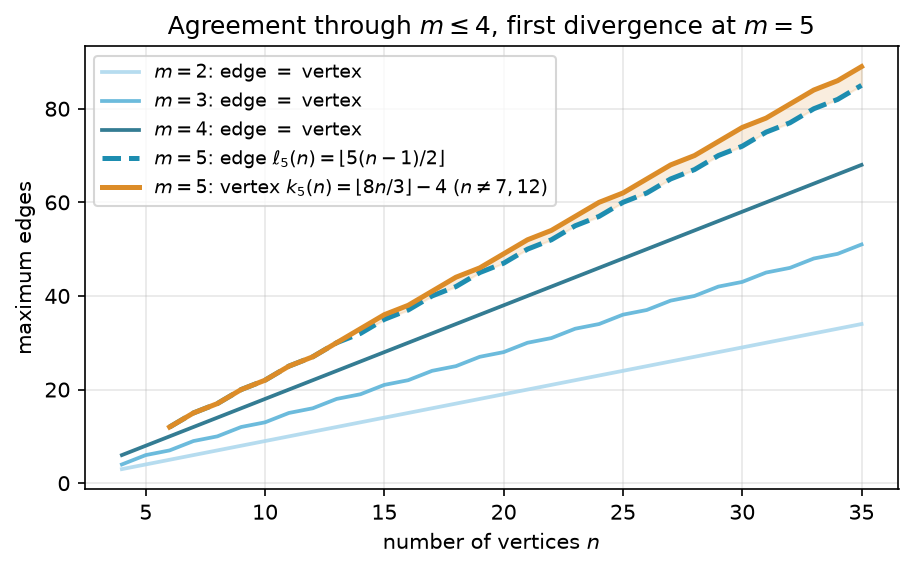
\includegraphics[width=\textwidth]{figures/edge_vertex_divergence.png}
    \caption{The edge and vertex extremal functions for $m = 2, 3, 4$ (blue shades, single curve per $m$ since they agree) and $m = 5$ (dashed blue for edge, solid orange for vertex). The vertex function diverges from the edge function at $n = 14$ and grows faster thereafter.}
    \label{fig:divergence}
\end{figure}

\begin{construction}[Directed hub]\label{const:directed-hub}
For $n \ge m \ge 2$, take a hub $h$ and label the other $N = n-1$ vertices $0, \dots, N-1$. Add the $2N$ hub arcs $h \to i$ and $i \to h$, and on the non-hub vertices the $(m-2)N$ ring arcs $i \to i+j \bmod N$ for $j = 1, \dots, m-2$. The total is $m(n-1)$ arcs and every non-hub vertex has $d^+ = d^- = m-1$.
\end{construction}

Every ordered pair has a non-hub member, whose relevant degree is exactly $m-1$ and, since $n \ge m$, smaller than the hub's own $n-1$. That member is therefore the binding one and the degree bound gives $\lec^{\max} \le m-1$. At $m = 2$ the ring is empty and what remains is the \emph{bidirected star}, in which two spokes can only reach each other through the hub.

\begin{construction}[One-directional bipartite digraph]\label{const:bipartite}
Split the vertices into parts $A$ and $B$ of sizes $\floor{n/2}$ and $\ceil{n/2}$, and include every arc from $A$ to $B$ and none the other way. The total is $\floor{n^2/4}$ arcs.
\end{construction}

Nothing leaves $B$ and nothing enters $A$, so no route has a second step and every pair is joined by at most the one direct arc, giving $\lec^{\max} = 1$.

\begin{theorem}[Directed arc value at $m = 2$]\label{thm:dir-arc-m2-exact}
For simple digraphs,
\[
    \ell_2^{\mathrm{dir}}(n) = \max\!\left(2(n-1),\ \floorfrac{n^2}{4}\right).
\]
\end{theorem}

The two constructions give the lower bound, one branch each. The upper bound is an induction on $n$ (\Cref{app:proofs}): delete a vertex of minimum total degree, which carries at most the average number of arcs, and apply the bound to what remains. The base cases $n \le 7$ are left to exhaustive search rather than hand argument, and \Cref{ch:machine} is what runs them. The same induction never mentions the separation, so it survives the change to $\kap$ verbatim once the base cases are re-run.

\begin{theorem}[Directed vertex value at $m = 2$]\label{thm:dir-vertex-m2-exact}
For simple digraphs, $k_2^{\mathrm{dir}}(n) = \ell_2^{\mathrm{dir}}(n)$.
\end{theorem}

\begin{figure}[h]
\centering
\begin{tikzpicture}[>=Stealth, scale=1.0,
    smallleftvertex/.style={gvertex}, smallrightvertex/.style={gvsink},
    hubvertex/.style={gvhub}, leftvertex/.style={gvertex},
    arc/.style={gdir},
    carc/.style={gdir, vertexorange!80!black}]

  % --- left panel: the bidirected star at n = 7, hub plus six spokes = 12 arcs ---
  \begin{scope}[shift={(-5.4,1.0)}, scale=0.92]
    \node[hubvertex, minimum size=7mm] (h) at (0,0) {$h$};
    \foreach \i/\ang in {0/90, 1/150, 2/210, 3/270, 4/330, 5/30} {
      \node[leftvertex, minimum size=7mm] (v\i) at (\ang:2.2) {$\i$};
    }
    \foreach \i in {0,...,5} {
      \draw[arc] (h) to[bend left=13] (v\i);
      \draw[arc] (v\i) to[bend left=13] (h);
    }
  \end{scope}
  % --- right panel: B_{3,4} at n = 7, every A-to-B arc = 12 arcs ---
  \begin{scope}[on background layer]
    \node[draw=KULblauw1!25, fill=KULblauw1!6, rounded corners=10pt,
          fit={(0,-0.6) (0,2.6)}, inner sep=8pt, minimum width=12pt] {};
    \node[draw=vertexred!25, fill=vertexred!6, rounded corners=10pt,
          fit={(4,-0.6) (4,2.6)}, inner sep=8pt, minimum width=12pt] {};
  \end{scope}
  \foreach \i in {1,...,3} {
    \node[smallleftvertex]  (a\i) at (0, {2.0-1.0*(\i-1)}) {$a_{\i}$};
  }
  \foreach \j in {1,...,4} {
    \node[smallrightvertex] (b\j) at (4, {2.5-1.0*(\j-1)}) {$b_{\j}$};
  }
  \foreach \i in {1,...,3} {
    \foreach \j in {1,...,4} {
      \draw[arc] (a\i) -- (b\j);
    }
  }
  \node[font=\small] at (0,-1.3) {$A$};
  \node[font=\small] at (4,-1.3) {$B$};
\end{tikzpicture}
\caption{The two branches tie at $n=7$, where each holds $12$ arcs at $\lec^{\max}=1$. Left: the bidirected star, a hub joined to six spokes both ways, $2(n-1)=12$. Right: the one-directional complete bipartite digraph $B_{3,4}$, every arc from $A$ to $B$, $\floor{n^2/4}=12$.}
\label{fig:simple-digraph-m2}
\end{figure}

The hub construction leads for $n < 7$, the one-directional bipartite construction leads for $n > 7$ and the two tie at $n = 7$, where both reach $12$ arcs. 
They are shown side by side in \Cref{fig:simple-digraph-m2}.
Notice how the directed value is quadratic in $n$ for large $n$, while the undirected value is linear.
This is because digraphs can be lopsided in one direction without creating routes back. 

\begin{proposition}[Hypergraph edge bound]\label{prop:hyper-edge}
An $r$-uniform hypergraph on $n$ vertices with Berge edge-connectivity at most $m-1$ has at most $\floorfrac{(m-1)(n-1)}{r-1}$ hyperedges. A simple hypergraph attains the bound whenever $m - 1 \le \binom{n-2}{r-2}$, and a multihypergraph attains it whenever $(r-1) \mid n - 1$.
\end{proposition}

The proof, given in \Cref{app:proofs}, runs the multigraph argument through the hypergraph Gomory-Hu theorem (\Cref{thm:hyper-gomory-hu} applied to the hyperedge-cut function in place of the edge-cut function, counting each hyperedge with the at least $r-1$ tree cuts it crosses. 
The star hypertree (\Cref{fig:hyper-star}) attains the $m = 2$ case, a hub joined to disjoint blocks of $r-1$ vertices, with Berge connectivity one everywhere and $\floor{(n-1)/(r-1)}$ hyperedges, exactly as a tree attained the multigraph bound. 
One genuine surprise is worth recording here: for $r \ge 3$ the bound is attained by \emph{simple} hypergraphs, with no repeated hyperedge, whenever $m-1\le\binom{n-2}{r-2}$ (\Cref{thm:simple-hyper-edge}). 
In the non-hypergraph case simplicity is exactly what separates Mader's $\floor{m(n-1)/2}$ from the multigraph value $(m-1)(n-1)$. 
One edge size higher, they are equal.

\begin{figure}[h]
\centering
\begin{tikzpicture}[scale=1.0,
   stn/.style={metrostop, minimum size=6mm},
   hub/.style={metrostop, minimum size=8.5mm, draw=vertexorange!90!black,
               fill=vertexorange!45, line width=1.4pt}]
  \coordinate (h) at (0,0);
  % two horizontal rows of four stations, the hub centred between them
  \coordinate (i1) at (-0.95, 1.3);  \coordinate (o1) at (-2.65, 1.3);
  \coordinate (i2) at ( 0.95, 1.3);  \coordinate (o2) at ( 2.65, 1.3);
  \coordinate (i3) at (-0.95,-1.3);  \coordinate (o3) at (-2.65,-1.3);
  \coordinate (i4) at ( 0.95,-1.3);  \coordinate (o4) at ( 2.65,-1.3);
  \begin{scope}[on background layer]
    % each hyperedge is one metro line: hub --(diagonal)-- inner --(horizontal)-- outer
    \draw[metro, metroA] (h) -- (i1) -- (o1);
    \draw[metro, metroB] (h) -- (i2) -- (o2);
    \draw[metro, metroC] (h) -- (i3) -- (o3);
    \draw[metro, metroD] (h) -- (i4) -- (o4);
  \end{scope}
  \foreach \p in {i1,o1,i2,o2,i3,o3,i4,o4} {\node[stn] at (\p) {};}
  \node[hub] at (h) {$h$};
\end{tikzpicture}
\caption{The $r=3$, $n=9$ star hypertree: four hyperedges meet only at the hub $h$, attaining $\floor{(n-1)/(r-1)}=4$ with Berge connectivity one.}
\label{fig:hyper-star}
\end{figure}

\begin{theorem}[Hypergraph vertex value at $m = 2$]\label{thm:hyper-vertex-m2}
For $r \ge 2$ and $n \ge 1$, the maximum number of hyperedges of an
$r$-uniform multihypergraph on $n$ vertices with $\kap^{\max} \le 1$ is
\[
    k_2^{(r)}(n) \;=\; \floorfrac{n-1}{r-1},
\]
attained by the star hypertree of \Cref{fig:hyper-star}. In particular
$k_2^{(r)}(n) = \ell_2^{(r)}(n)$: the vertex and edge problems agree at $m = 2$
for every uniformity, and repeated hyperedges never help.
\end{theorem}

\begin{theorem}[Hypergraph vertex value at $m = 3$]\label{thm:hyper-vertex-m3}
For $r \ge 2$, every $r$-uniform multihypergraph on $n$ vertices with
$\kap^{\max} \le 2$ has at most $\floorfrac{2(n-1)}{r-1}$ hyperedges. For
$r \ge 3$ with $2 \le \binom{n-2}{r-2}$ the bound is attained by a simple
hypergraph, so
\[
    k_3^{(r)}(n) \;=\; \floorfrac{2(n-1)}{r-1} \;=\; \ell_3^{(r)}(n).
\]
\end{theorem}

The first falls out once Berge routes are read as ordinary paths in the incidence graph, where the ceiling $\kap^{\max} \le 1$ says exactly that the incidence graph is a forest. 
The second is the harder one and carries the genuinely new tool: a rank bound for graphs in which one side of a partition must stay below local $3$-connectivity, proved by way of Tutte's triconnected decomposition, which the incidence translation then turns back into the hypergraph statement. 
At $m \ge 4$ that route stops for want of a $4$-connectivity analogue of the decomposition, and the value is open.
The proposition counts hyperedges, but it does not say how to \emph{measure} the Berge connectivity of a hypergraph we are handed and that measurement is the genuinely new part. 
The metro picture shows why. 
An ordinary edge is a one-stop link between a single pair, so policing edge-disjointness means watching each pair on its own. 
A hyperedge is a whole line: it stops at all $r$ of its vertices and so touches $\binom{r}{2}$ pairs at once, yet like a line that can run only one train at a time it may serve only one route. 
When several routes want to board the same line at different stations, the checker must wave exactly one through and turn the rest away and it must do this for every line simultaneously. 
That bookkeeping is the one new piece of machinery the next chapter builds and it is why the hypergraph rejoins the family only once the checker is in place.


\section{Conjectured bounds}

\begin{conjecture}\label{conj:dir-arc}
For simple digraphs and all $n \ge m \ge 2$,
\[
    \ell_m^{\mathrm{dir}}(n) = \max\!\left(m(n-1),\ \floorfrac{(n+m-2)^2}{4}\right).
\]
\end{conjecture}

At $m = 2$ this is \Cref{thm:dir-arc-m2-exact}. The first branch is the directed hub. The second is the bipartite digraph with one extra layer inside its larger part.

\begin{construction}[Augmented bipartite digraph]\label{const:augmented-bipartite}
For $n \ge m \ge 2$, set $|B| = \ceil{(n+m-2)/2}$ and $|A| = n - |B|$, include every arc from $A$ to $B$, and inside $B$ give each $b_j$ the $m-2$ in-arcs from its cyclic predecessors $b_{j-1}, \dots, b_{j-(m-2)}$. The total is $\floor{(n+m-2)^2/4}$ arcs.
\end{construction}

The only in-arcs of a $b \in B$ that an $a \in A$ can reach are the direct arc $a \to b$ and the $m-2$ two-step detours through $b$'s in-neighbours inside $B$, so such a pair carries exactly $m-1$ routes and no more, while pairs inside $B$ are held down by the in-degree $m-2$ and pairs from $B$ to $A$ or inside $A$ have no routes at all.

At $m = 3$, $n = 10$ this is the digraph that refutes the natural first guess $\max(m(n-1), \floor{n^2/4})$. Its $25$ arcs from $A$ to $B$ carry a five-cycle inside $B$, giving every $b_j$ one extra in-arc, so each pair $a_i, b_j$ has the direct arc and one detour and $\lec^{\max} = 2$. That is $30$ arcs against the guess of $27$, and the correction is exactly the shift of the partition towards $B$.

For fixed $m \ge 3$ the matching upper bound is open, though not entirely: \Cref{thm:dir-arc-linear-error} proves unconditionally that the value is $n^2/4 + \Theta_m(n)$, so what the conjecture still claims beyond what is known is the coefficient of the linear term rather than the shape of the answer.








% move all of this to the appendix. 
% \begin{construction}[Directed hub]\label{const:directed-hub}
% For $n \ge m \ge 2$, take a hub vertex $h$ and label the remaining $N = n - 1$ vertices $0, 1, \dots, N-1$. Add the $2N$ hub arcs $h \to i$ and $i \to h$ for every $i$, and on the non-hub vertices add the circulant arcs $i \to i + j \pmod{N}$ for $j = 1, \dots, m-2$, the target label wrapping around past $N$ back to $0$ (that ring pattern is what \emph{circulant} means, and ``$\bmod\ N$'' is the wrap-around). Counting these gives $2N$ hub arcs (each of the $N$ spokes joined to $h$ in both directions) plus $(m-2)N$ circulant arcs ($m-2$ layers, one arc per spoke), so the total is $2N + (m-2)N = mN = m(n-1)$ arcs. Every non-hub vertex has $d^+ = d^- = 1 + (m-2) = m-1$. Every ordered pair $(u,v)$ has at least one non-hub member, and that member's relevant degree is exactly $m-1$, smaller than the hub's own degree $n-1$ since $n \ge m$, so it is always the binding one regardless of which of $u,v$ is the hub. The directed degree bound (\Cref{lem:degree-bound}, which says $\lec(u,v)\le\min(d^+(u),d^-(v))$, since a route out of $u$ must use one of $u$'s out-arcs and one of $v$'s in-arcs) therefore gives $\lec^{\max} \le m-1$.
% \end{construction}
% At $m = 2$ this construction is easiest to picture: the circulant layer is empty and what remains is the \emph{bidirected star} of \Cref{fig:bidirected-star}, a hub joined to each spoke by a matched pair of opposite arcs. Every spoke can reach every other only by going in to the hub and back out, two hops, so no pair is ever joined by two independent routes, and the arc total is exactly $2(n-1)$. For $m \ge 3$ not all $m(n-1)$ arcs can touch the hub, since a simple digraph has at most $2(n-1)$ arcs incident to one vertex: the surplus lives in the circulant layers among the spokes, tuned so that no degree exceeds the budget. The two constructions compete on different scales, linear against quadratic, and which one wins depends on $n$. At $m = 2$ the competition resolves exactly.

% % --- right panel: m = 3 (hub + one circulant layer among spokes) ---
%   \begin{scope}[shift={(3.2,0)}, scale=0.92]
%     \node[hubvertex, minimum size=7mm] (H) at (0,0) {$h$};
%     \foreach \i/\ang in {0/90, 1/150, 2/210, 3/270, 4/330} {
%       \node[leftvertex, minimum size=7mm] (u\i) at (\ang:2.2) {$\i$};
%     }
%     % hub arcs (blue, both directions)
%     \foreach \i in {0,...,4} {
%       \draw[arc] (H) to[bend left=13] (u\i);
%       \draw[arc] (u\i) to[bend left=13] (H);
%     }
%     % single circulant layer j=1: i -> (i+1) mod 5  (orange), bowed outward
%     \foreach \i/\j in {0/1, 1/2, 2/3, 3/4, 4/0} {
%       \draw[carc] (u\i) to[bend right=22] (u\j);
%     }
%     \node[font=\small, text=black!70] at (0,-3.0) {$m=3$, $n=6$: $m(n{-}1)=15$ arcs};
%   \end{scope}
% \paragraph{Idea of the upper bound at $m = 2$.} Which of the two branches of $M(n) = \max(2(n-1), \floor{n^2/4})$ leads is pure arithmetic: $2(n-1) \ge \floor{n^2/4}$ precisely for $n \le 7$, with equality at $n = 7$, where both give $12$. So $M$ follows the bidirected star up to the crossover and the bipartite digraph past it, and $n = 7$ is the single size at which the two constructions tie. That no digraph beats $M(n)$ is an induction on $n$, carried out in \Cref{app:proofs}. Delete a vertex of \emph{minimum} total degree. Two facts about that deletion meet. The degrees sum to twice the arc count, so the deleted vertex carries at most the average $2a/n$ arcs, and what remains still respects the ceiling, so the inductive bound applies to it. Feeding both into the split of the arc count leaves a copy of $a$ on each side, and gathering them yields $a \le \tfrac{n}{n-2}\floor{(n-1)^2/4}$, which a parity check shows never exceeds $\floor{n^2/4}$ once $n \ge 8$. Nothing in the argument is deep. It is a careful walk through two parity regimes, with the base cases $n \le 7$ settled by exhaustive computer search rather than by hand. That experience of a correct but long and almost entirely mechanical case-check is exactly what motivates the chapters that follow. One genuinely wants to hand the case-checking to a machine.

% The vertex-disjoint version of the same question has the same answer at $m = 2$, but it is worth being careful about why, because Whitney's inequality is easy to read backwards here. Since $\kap \le \lec$ pairwise, a digraph that respects the arc ceiling automatically respects the vertex one, so the vertex-feasible family \emph{contains} the arc-feasible one and is in general strictly larger. The free consequence therefore runs one way only: the two constructions above keep $\kap^{\max} = 1$ as readily as $\lec^{\max} = 1$, which makes them lower bounds for the vertex problem too. No upper bound comes with them. What settles the vertex value is that the same induction goes through unchanged, because deleting a vertex lowers $\kap^{\max}$ for exactly the reason it lowers $\lec^{\max}$, and because the base cases $n \le 7$ were re-run under the stricter separation and returned the same six numbers. \Cref{app:proofs} gives both halves, and \Cref{rem:whitney-direction} there spells out the direction trap in full.


% \subsection{The failure of direct proof for \texorpdfstring{$m \ge 3$}{m >= 3}}
% For $m \ge 3$ the induction no longer closes, and the natural guess is wrong. The natural initial conjecture was that the two constructions above continued to be the whole story, giving $\max(m(n-1), \floor{n^2/4})$. A single graph on ten vertices refutes it.

% \begin{remark}[A thirty-arc counterexample]\label{rem:counterexample-m3}
% Take $A = \{a_1, \dots, a_5\}$ and $B = \{b_1, \dots, b_5\}$ with all $25$ arcs from $A$ to $B$, and add a directed five-cycle $b_1 \to b_2 \to b_3 \to b_4 \to b_5 \to b_1$ inside $B$. This digraph has $30$ arcs. Every vertex of $B$ has exactly one extra in-arc from inside $B$, so two arc-disjoint routes from $a_i$ to $b_j$ exist: the direct arc $a_i \to b_j$, and the detour $a_i \to b_{j-1} \to b_j$ using the 5-cycle predecessor of $b_j$ (indices mod 5). For the matching upper bound, the only in-arcs of $b_j$ reachable on a path from $a_i$ are the direct arc $a_i \to b_j$ and the cycle arc $b_{j-1} \to b_j$. Removing both disconnects $a_i$ from $b_j$, while neither alone does, so the minimum cut has size 2. Hence $\lec(a_i, b_j) = 2$. Routes between two vertices of $B$ never leave $B$ and give $\lec(b_i, b_j) = 1$. Hence $\lec^{\max} = 2$, so the graph is feasible at $m = 3$, yet $30 > \max(3 \cdot 9,\ 25) = 27$.
% \end{remark}

% \Cref{fig:augmented-bipartite} draws this thirty-arc digraph and traces the mechanism. The twenty-five faint arcs are the complete one-directional bipartite layer from $A$ to $B$, the construction we already understand. On top of them the orange five-cycle gives each vertex of $B$ a single extra in-arc from inside $B$. That one extra arc is exactly what doubles the connectivity. For the marked pair $a_1, b_2$ the two heavy routes show how: the blue arc is the direct hop $a_1 \to b_2$, and the green path $a_1 \to b_1 \to b_2$ borrows the cycle arc $b_1 \to b_2$ for its second step. The two share no arc, so $\lec(a_1, b_2) = 2$, and the same pair of routes exists for every $a_i, b_j$. Five extra arcs lift the whole digraph from one independent route per pair to two, and the thirty arcs overshoot the old prediction of twenty-seven.

% \begin{figure}[ht]
% \centering
% \begin{tikzpicture}[>=Stealth, scale=1.05,
%     smallleftvertex/.style={gvertex}, smallrightvertex/.style={gvsink},
%     bgarc/.style={gdirfaint},
%     directarc/.style={grBd, KULblauw1},
%     detourarc/.style={grBd, vertexgreen!75!black},
%     cycarc/.style={-{Stealth[length=1.8mm]}, line width=1.2pt, vertexorange!90!black, line cap=round}]
%   \foreach \i in {1,...,5} {
%     \node[smallleftvertex]  (a\i) at (0, {2.4-1.05*(\i-1)}) {$a_{\i}$};
%   }
%   \foreach \i in {1,...,5} {
%     \node[smallrightvertex] (b\i) at (4.0, {2.4-1.05*(\i-1)}) {$b_{\i}$};
%   }
%   % faint complete bipartite background (all 25 arcs)
%   \foreach \i in {1,...,5} {
%     \foreach \j in {1,...,5} {
%       \draw[bgarc] (a\i) -- (b\j);
%     }
%   }
%   % directed 5-cycle inside B, on the right
%   \foreach \i/\j in {1/2,2/3,3/4,4/5} {
%     \draw[cycarc] (b\i) to[bend left=58] (b\j);
%   }
%   \draw[cycarc] (b5) to[bend left=30] (b1);
%   % highlight the two arc-disjoint routes a1 -> b2 :
%   %  direct a1 -> b2 ;  detour a1 -> b1 -> b2 through the cycle arc
%   \draw[directarc] (a1) -- (b2);
%   \draw[detourarc] (a1) -- (b1);
%   \draw[detourarc] (b1) to[bend left=58] (b2);
%   \node[font=\small] at (0,-3.3) {part $A$};
%   \node[font=\small] at (4.0,-3.3) {part $B$};
% \end{tikzpicture}
% \caption{The thirty-arc counterexample at $m=3$, $n=10$: $25$ arcs run from $A$ to $B$ and a directed $5$-cycle lies inside $B$. The highlighted direct route and detour show the binding value $\lec^{\max}=2$.}
% \label{fig:augmented-bipartite}
% \end{figure}

% The counterexample generalises: the five-cycle gave every vertex of $B$ exactly one extra in-arc from inside $B$, and the budget for such arcs is $m - 2$ per vertex, not one. \Cref{fig:augmented-bipartite} is the instance $m = 3$, where that budget is one and a single cycle suffices. For larger $m$ each $b_j$ collects $m - 2$ cyclic predecessors and the same picture acquires more concentric chords inside $B$.

% \begin{construction}[Augmented bipartite digraph]\label{const:augmented-bipartite}
% For $m \ge 2$ and $n \ge m$, set $|B| = \ceil{(n+m-2)/2}$ and $|A| = n - |B| = \floor{(n-m+2)/2}$, include every arc from $A$ to $B$, and inside $B$ give each vertex $b_j$ the $m-2$ in-arcs from its cyclic predecessors $b_{j-1}, \dots, b_{j-(m-2)}$ (indices mod $|B|$). The total is $\floor{(n+m-2)^2/4}$ arcs.

% Its arc count is the product of the two halves of $n+m-2$, and its connectivity is verified in \Cref{app:proofs}. The point there is that the only in-arcs of a $b \in B$ that any $a \in A$ can reach are the direct arc $a \to b$ and the $m-2$ two-step detours through $b$'s in-neighbours inside $B$, so each such pair carries exactly $m-1$ arc-disjoint routes and no more, while pairs inside $B$ are held down by the in-degree $m-2$, and pairs from $B$ to $A$ or inside $A$ have no routes at all.

% At $m = 2$ the inside of $B$ is empty and the construction reduces to \Cref{const:bipartite}, with the balanced partition $(\floor{n/2}, \ceil{n/2})$. At $m = 3$ the formula gives $|B| = \ceil{(n+1)/2}$, which coincides with $\ceil{n/2}$ at odd $n$ but gives $|B| = n/2 + 1$ at even $n$. Both the balanced and the shifted partition achieve the same arc count $\floor{n^2/4} + \ceil{n/2}$ in this case, so the two are interchangeable at $m = 3$. The shift to a strictly larger $B$ is structurally significant only at $m \ge 4$, where the balanced partition is suboptimal. At $m = 3$, $n = 10$ it is the thirty-arc counterexample of \Cref{rem:counterexample-m3}, drawn in \Cref{fig:augmented-bipartite} (using the equivalent balanced partition $|A| = |B| = 5$).
% \end{construction}

% The two rival shapes invite a political picture. The hub is a single king through whom all traffic must pass, cheap to build but limited by the one throne. The bipartite family is a flat cabinet of ministers, each handling its own dossier with no central seat, and it scales quadratically. Which arrangement packs more arcs under the ceiling depends on $n$, and for $m \ge 3$ the cabinet overtakes the king once $n$ is large. This is the corrected shape, and it leads to the standing conjecture for the directed arc problem.



% The hypothesis $n \ge m$ is the one both constructions already carry, and it is needed for the same reason as in \Cref{thm:leonard}: below it the complete digraph is feasible and the answer is the trivial $n(n-1)$, which the formula exceeds. At $n = 3$, $m = 4$ the formula gives $8$ where three vertices carry only $6$ arcs. The exhaustive search confirms the value is $6$ there.

% For $m = 2$ this is \Cref{thm:dir-arc-m2-exact}. For $m = 3$ the formula $\floor{(n+1)^2/4}$ equals $\floor{n^2/4} + \ceil{n/2}$, so the conjecture reduces to the previous formula for $m = 2$ and $m = 3$. For $m = 3$, $n = 10$ the second branch gives $\floor{121/4} = 30$, matching \Cref{rem:counterexample-m3}. For $m \ge 4$ the new formula and the old balanced-partition count $\floor{n^2/4} + (m-2)\ceil{n/2}$ no longer agree. The quadratic branches already differ, and at $m = 4$ the new one is larger by exactly one at every even $n$. At small $n$, though, the hub term $m(n-1)$ dominates both branches and hides that difference. The full conjectured value therefore first overtakes the old one only at $n = 12$, for $m = 4$. The construction of \Cref{const:augmented-bipartite} with the shifted partition witnesses the difference. The lower bound holds for all $m$, witnessed by \Cref{const:directed-hub} on the first branch and \Cref{const:augmented-bipartite} on the second. For fixed $m\ge3$, the matching upper bound is open, though not entirely: \Cref{thm:dir-arc-linear-error} proves unconditionally that the value is $n^2/4 + \Theta_m(n)$, so what the conjecture still claims beyond what is known is the coefficient of that linear term rather than the shape of the answer. \Cref{ch:synthesis} returns to it with what structural progress the machine and the hand can jointly supply.

% \section{The hypergraph variant}
% The third model deserves its own short treatment, not because its base case is hard but because it is the one variant whose objects are stored and manipulated differently from all the rest, and it is worth meeting that difference now rather than at the moment of computation. A hypergraph keeps no multiplicity matrix, only the list of its hyperedges, each a set of $r$ vertices. We fix the edge size $r$, following the extremal literature, for a structural reason: under a connectivity ceiling a small edge is always at least as efficient per route as a large one, so a hypergraph free to mix sizes would maximise its edge count by using pairs only, and the question would collapse back to the graph case. Fixing $r$ is what makes the hypergraph question a new question.

% The route between two vertices is a \emph{Berge path}, which alternates vertices and hyperedges so that each consecutive pair of vertices lies in the hyperedge listed between them, and two such routes are edge-disjoint when they share no hyperedge. Concretely, in a three-uniform hypergraph a route from $u$ to $w$ might be the single step $u, \{u, x, w\}, w$ that crosses one hyperedge, or a longer alternation $u, \{u, x, y\}, y, \{y, z, w\}, w$ that switches hyperedge at the intermediate vertex $y$.

% With routes redefined this way the same Gomory--Hu machinery that proved the multigraph value carries over, and the base case has the same linear shape. The picture to keep in mind is a metro map: each hyperedge is a line, and a route from one vertex to another rides a line and changes to another line at a station the two share.

% A single hyperedge may serve only one route, so two Berge routes that share no hyperedge are edge-disjoint, the hypergraph counterpart of two edge-disjoint paths in a graph. In the metro picture, two hyperedges that share several vertices are distinct lines calling at several of the same stations, as in \Cref{fig:four-models}. Two routes are hyperedge-disjoint exactly when they never ride the same line.

% This is one of several inequivalent notions of hypergraph connectivity, and the choice matters, so it is worth saying which one is meant. Dewar, Pike and Proos \cite{DewarPikeProos18} survey the competing definitions and how they separate, and Berge routes with hyperedge-disjointness are the notion used throughout here, matching Berge's own \cite{Berge89}. The dual cut side is the hyperedge cut, whose minimisation is studied algorithmically by Chekuri and Xu \cite{ChekuriXu17}, and it is exactly the quantity the checker of \Cref{ch:machine} computes and the hypergraph Gomory--Hu tree of \Cref{thm:hyper-gomory-hu} organises.

% The separation axis needs its own definition here, and it is worth fixing now because the natural guess is not the one this thesis uses. Two Berge routes are called \emph{internally disjoint} when they share neither an intermediate vertex nor a hyperedge. Both halves are required. Demanding only that the routes avoid each other's intermediate stations would let two routes ride the same line, and a line that can run only one train at a time cannot serve two routes at once, so the resulting count would not correspond to anything the metro map can carry. Requiring both is also what makes the vertex measure the exact analogue of the graph one under the translation of \Cref{app:proofs}, where a hypergraph becomes its incidence graph, each hyperedge becomes a node, and internally disjoint routes become internally disjoint paths in the ordinary sense. It has the pleasant side effect that Whitney's inequality survives the move to hypergraphs by definition, since an internally disjoint family is in particular hyperedge-disjoint. Write $\kap_\HH(u,v)$ for the largest such family and $\kap^{\max}_\HH$ for its maximum over pairs.


% The edge bound is the easy half of the hypergraph story. The vertex separation is where this thesis has something new to say, and its two statements are worth having in front of the reader before the machinery that establishes them.

% all of this seems boring, i'd prefer you take what is needed to be mentioned: what parts of the implementation i actually should refer to, but that belongs in the next chapter. 
% \section{Where this work sits}
% %seems repetitive and not needed, 
% % It is worth pausing, before the machine, to place the question and the method against the two traditions they descend from: the extremal graph theory that posed the problem and the computational mathematics that will help settle it.

% % The mathematical lineage is the older of the two. The problem belongs to the family of extremal connectivity questions opened by Bollob\'{a}s and Erd\H{o}s, who asked how dense a graph can be while every pair of vertices stays below a fixed connectivity \cite{BollobasErdos62}, logged today as Erd\H{o}s Problem 915 \cite{ErdosProblems}. Mader's theorem \cite{Mader73} closed the simple undirected edge case with the clean floor $\floor{m(n-1)/2}$ recalled in \Cref{thm:mader}, and it is the floor every variant in this thesis is measured against. The vertex-disjoint branch has a longer and rougher history. Leonard \cite{Leonard72b} showed that the edge and vertex problems coincide through $m \le 4$, and S\o{}rensen and Thomassen \cite{SorensenThomassen74} found the first divergence at $m = 5$, where $k_5(n) = \floor{8n/3} - 4$ for every $n \ge 6$ except $n = 7$ and $n = 12$ (whose values are $15$ and $27$). Past that point the exact values $k_m(n)$ remain unknown. What is known there is one negative and one bound: the original conjecture of Bollob\'{a}s and Erd\H{o}s is false for every $m \ge 6$ \cite{Mader73}, and a general lower bound is available \cite{SorensenThomassen74}. That gap between a settled edge case and a stalled vertex case is exactly the terrain \Cref{ch:basecases} has been mapping, and the directed and hypergraph axes extend it further. To this particular lineage, the undirected vertex problem, the thesis adds no new closed form. It does add exact formulas and asymptotic results on the directed and hypergraph axes.

% The computational tradition this thesis's pipeline belongs to is the practice of settling combinatorial questions by machine in a way a human can audit, and it splits into a few schools worth contrasting with the certify-then-prove loop built next. The oldest is \emph{exhaustive generation}: enumerate every object of a given size up to isomorphism and check each one. McKay and Piperno's \texttt{nauty}/\texttt{geng} toolkit \cite{McKayPiperno14} is the standard engine for this, and its flagship results include exact small Ramsey numbers such as $R(4,5) = 25$ \cite{McKayRadziszowski95}. The enumeration of \Cref{ch:certify} is the same idea, run on the twelve variants of Problem 915. The second school is \emph{SAT-assisted proof}, in which a question is encoded in propositional logic and a solver emits a machine-checkable certificate. Two results are the canonical examples of certified solver output at scale: Heule, Kullmann and Marek's resolution of the Boolean Pythagorean triples problem \cite{HeuleKullmannMarek16}, whose verified proof runs to some two hundred terabytes, and Heule's determination of Schur number five \cite{Heule18}. The third is \emph{flag algebras}, Razborov's framework \cite{Razborov07} that converts asymptotic extremal bounds into semidefinite-programming certificates, the dominant tool for density problems in the large-$n$ limit. Closest of all to the method here is the fourth, \emph{certification by linear and integer programming} (LP/ILP). A feasibility or optimality argument over the rationals or integers is written as a linear program, meaning an optimisation whose constraints are all linear. Such a solve can in principle be accompanied by primal and dual data that a separate checker verifies. The cut-counting optimisation of \Cref{ch:certify} records the solver's status and an integral primal witness, but does not emit that independently replayable certificate. \Cref{sec:certification-standard} states the evidential standard used here.

% Against that backdrop, what is distinctive here is consolidation rather than a new solver. A single program measures connectivity exactly across all twelve problem variants through one common interface, using a matrix representation for graphs and a separate compact representation for hypergraphs, so search and certification share one codebase rather than living in separate tools. Its connectivity outputs and witnesses are exact integral objects. An optimiser's \texttt{OPTIMAL} status is recorded as machine evidence and is not presented as a formal certificate by itself. The general statements that use those finite values also have the independent hand proofs in \Cref{app:proofs}. Because the same program both hunts for dense graphs and checks the bounds they suggest, the discover and finite-verification steps are two modes of one loop. What makes the consolidation honest is that it never blurs three kinds of knowledge: a value can be \emph{proved} (by hand or exhaustive enumeration), \emph{solver-verified} at a finite size, or only \emph{conjectured} (witnessed by a dense graph with no matching upper bound). This trichotomy, named in \Cref{sec:trichotomy} and obeyed by the summary of \Cref{ch:synthesis}, is the through-line of everything that follows.

% \begin{computernote}
% We are now stuck in three different ways: a fifty-year-old open problem at $m \ge 6$ for vertices, a long proof we would rather not check by hand at $m = 2$ for arcs, and at $m \ge 3$ a conjecture of which only the leading behaviour can be proved. The base cases of the long induction were verified by exhaustive search. The thirty-arc counterexample was not: ten vertices put a blind sweep of digraphs far out of reach, so it was constructed and then confirmed pair by pair by the same exact checker. The next chapter builds a single program that models all of these cases at once, measures their connectivity exactly, and proves the small-case upper bounds outright.
% \end{computernote}
